% Options for packages loaded elsewhere
\PassOptionsToPackage{unicode}{hyperref}
\PassOptionsToPackage{hyphens}{url}
%
\documentclass[
]{book}
\usepackage{amsmath,amssymb}
\usepackage{lmodern}
\usepackage{iftex}
\ifPDFTeX
  \usepackage[T1]{fontenc}
  \usepackage[utf8]{inputenc}
  \usepackage{textcomp} % provide euro and other symbols
\else % if luatex or xetex
  \usepackage{unicode-math}
  \defaultfontfeatures{Scale=MatchLowercase}
  \defaultfontfeatures[\rmfamily]{Ligatures=TeX,Scale=1}
\fi
% Use upquote if available, for straight quotes in verbatim environments
\IfFileExists{upquote.sty}{\usepackage{upquote}}{}
\IfFileExists{microtype.sty}{% use microtype if available
  \usepackage[]{microtype}
  \UseMicrotypeSet[protrusion]{basicmath} % disable protrusion for tt fonts
}{}
\makeatletter
\@ifundefined{KOMAClassName}{% if non-KOMA class
  \IfFileExists{parskip.sty}{%
    \usepackage{parskip}
  }{% else
    \setlength{\parindent}{0pt}
    \setlength{\parskip}{6pt plus 2pt minus 1pt}}
}{% if KOMA class
  \KOMAoptions{parskip=half}}
\makeatother
\usepackage{xcolor}
\IfFileExists{xurl.sty}{\usepackage{xurl}}{} % add URL line breaks if available
\IfFileExists{bookmark.sty}{\usepackage{bookmark}}{\usepackage{hyperref}}
\hypersetup{
  pdftitle={데이터 시각화},
  pdfauthor={한국 R 사용자회},
  hidelinks,
  pdfcreator={LaTeX via pandoc}}
\urlstyle{same} % disable monospaced font for URLs
\usepackage{longtable,booktabs,array}
\usepackage{calc} % for calculating minipage widths
% Correct order of tables after \paragraph or \subparagraph
\usepackage{etoolbox}
\makeatletter
\patchcmd\longtable{\par}{\if@noskipsec\mbox{}\fi\par}{}{}
\makeatother
% Allow footnotes in longtable head/foot
\IfFileExists{footnotehyper.sty}{\usepackage{footnotehyper}}{\usepackage{footnote}}
\makesavenoteenv{longtable}
\usepackage{graphicx}
\makeatletter
\def\maxwidth{\ifdim\Gin@nat@width>\linewidth\linewidth\else\Gin@nat@width\fi}
\def\maxheight{\ifdim\Gin@nat@height>\textheight\textheight\else\Gin@nat@height\fi}
\makeatother
% Scale images if necessary, so that they will not overflow the page
% margins by default, and it is still possible to overwrite the defaults
% using explicit options in \includegraphics[width, height, ...]{}
\setkeys{Gin}{width=\maxwidth,height=\maxheight,keepaspectratio}
% Set default figure placement to htbp
\makeatletter
\def\fps@figure{htbp}
\makeatother
\setlength{\emergencystretch}{3em} % prevent overfull lines
\providecommand{\tightlist}{%
  \setlength{\itemsep}{0pt}\setlength{\parskip}{0pt}}
\setcounter{secnumdepth}{5}
\ifLuaTeX
  \usepackage{selnolig}  % disable illegal ligatures
\fi

\title{데이터 시각화}
\author{한국 R 사용자회}
\date{2022-05-04}

\begin{document}
\maketitle

{
\setcounter{tocdepth}{1}
\tableofcontents
}
\hypertarget{uxb370uxc774uxd130-uxc2dcuxac01uxd654}{%
\chapter*{데이터 시각화}\label{uxb370uxc774uxd130-uxc2dcuxac01uxd654}}
\addcontentsline{toc}{chapter}{데이터 시각화}

\begin{center}\rule{0.5\linewidth}{0.5pt}\end{center}

후원계좌

디지털 불평등 해소를 위해 제작중인 오픈 통계패키지 개발과 고품질 콘텐츠 제작에 큰 힘이 됩니다.

\begin{verbatim}
  - 하나은행 448-910057-06204
  - 사단법인 한국알사용자회
\end{verbatim}

\hypertarget{happy-viz}{%
\chapter{행복한 시각화}\label{happy-viz}}

캐나다 브리티쉬 콜럼비아 대학 \href{https://stat545.com/}{STAT545} 교육과정이 공개되어
초창기 데이터 과학이 정립될 때 큰 역할을 하였다.
``행복한 시각화 생활을 위한 비밀'' 장에 성공적인 시각화를 핵심적인 내용이 담겨있다.

시각화 그래프를 제작하는데 어려움이 있다면,
\texttt{ggplot2} 코드에 문제가 있다고 시각화 관련 부분에 집중적인 시간을 투여할 것이다.
하지만 다음 세가지 지점을 먼저 살펴봐라.

\begin{itemize}
\tightlist
\item
  데이터프레임에 시각화 관련 작업을 담아둔다.
\item
  데이터프레임을 \emph{깔끔하게(tidy)} 제작한다; 시각화에 적절한 자료형으로 변환
\item
  범주형(factor) 변수를 적절히 활용함은 물론 범주형 자료 장인이 된다.
\end{itemize}

나중에 심도있게 다룰 시각화 자료구조인 깔끔한 \textbf{데이터(Tidy Data)}를 제작하게 되면
그동안 자신을 괴롭혔던 시각화 관련 문제는 자연히 사라져 버린다.
이를 위해서 \texttt{dplyr} 패키지의 데이터 다루는 여러 동사를 \texttt{tidyr} 패키지
깔끔한 데이터 제작 동사와 결합하여 사용하게 되면 생산성을 크게 높일 수 있다.

\hypertarget{viz-secret-dataframe}{%
\section{시각화 입력 자료구조: 데이터프레임}\label{viz-secret-dataframe}}

기억해야 할 단 한가지 사항은 시각화 자료구조는 데이터프레임이다.
좀더 구체적으로 \textbf{깔끔한 데이터}다.
시각화 산출물을이 동일하다고 하더라도 작성한 코드를 면밀히 살펴보면
가독성이 떨어짐은 물론 \texttt{tidyverse} 관습과 동떨어진 경우를 종종 보게 된다.

예를 들어, 많은 경우 변수가 데이터프레임 밖에 복사되어
작업공간에 독립된 객체로 존재시켜 이를 시각화하는 것이다.

앞선 방식의 문제는 \texttt{ggplot2} 패키지로 시각화가 되지 않고 오류가 발생된다.
근본 원인은 \texttt{ggplot2} 패키지 \texttt{ggplot()} 함수가 입력값이 데이터프레임이라는데 있다.
즉, 데이터프레임을 입력받아 시각화 그래프를 출력으로 뱉어내는데 이를 충족시키지 못할 경우
의도한 바가 컴퓨터에 전달되지 않아 오류가 나와 더이상 진전을 이룰 수가 없다.

즉, 변수를 데이터프레임에 담아 보관하고 \texttt{ggplot()} 함수에 시각화 대상 데이터프레임에 전달하면 된다.
이런 전략은 R에 존재하는 다른 시각화 플랫폼에도 동일하게 적용된다.
R에는 \texttt{ggplot}을 비롯하여 Base 그래픽, \texttt{lattice} 그래픽 등 크게 3가지가 존재한다.
모두 방식에는 다소 차이가 있지만 근본적으로 데이터프레임을 입력받아 시각화 그래프를 출력으로 내보낸다.

파이프 연산자를 사용해서 좀더 직관적으로 코드를 다음과 같이 제작하게 되면
의미가 명확해질 것이다.

\begin{center}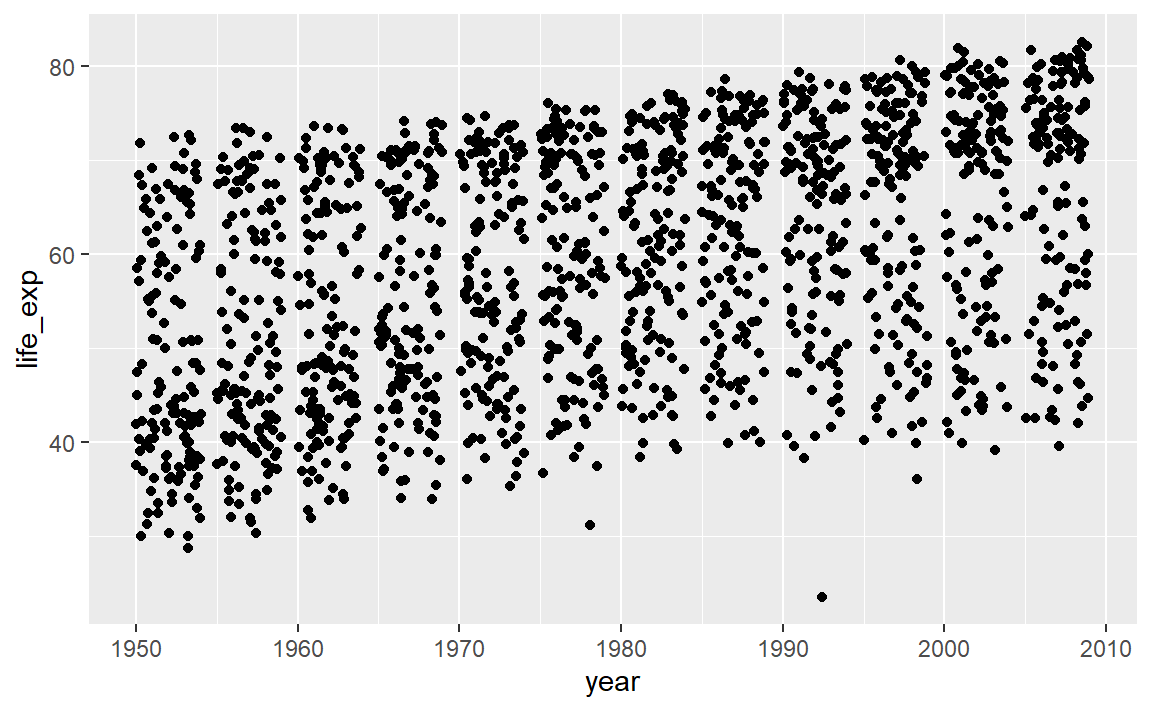
\includegraphics{happy-visualization_files/figure-latex/data-in-situ-1} \end{center}

예를 들어 시각화 대상이 국가별, 대륙별, 년도별 데이터를 필터링하는 경우도 있다.
관련 모든 변수가 데이터프레임에 있게되면 훨씬 더 쉽고 안전하게 작업을 수행할 수 있다.
앞서 시각화 변수를 별도 작업공간(메모리)에 별도 저장하여 관리할 경우 대비하여
생각하게 되면 데이터프레임에 시각화 모든 정보를 담아두는 전략의 명확한 우위가 드러난다.

\texttt{ggplot2} 시각화 시스템만 데이터프레임을 받아 시각화하는 유일한 특이한 사례는 아니다.
데이터프레임에 모든 정보를 담아두고 필요한 경우 \texttt{dplyr} 동사로 변수생성, 필터링,
그룹별 요약, 정렬 등 데이터 조작 작업을 통해 시각화 대상 데이터프레임을 만들고
이를 시각화하는 전략은 널리 인정되는 모범사례다.

데이터프레임을 \texttt{data=} 선택옵션으로 전달하는 것이 많이 사용되는 R 함수에 일반적인 기능이다.
예를 들어, \texttt{lm()}, \texttt{aggregate()}, \texttt{plot()}, \texttt{t.test()}.
따라서, 이런 방식이 기본디폴트 작업방식이 된다.

\hypertarget{viz-secret-explicit-dataframe}{%
\section{\texorpdfstring{\texttt{dplyr::data\_frame()} 자료구조}{dplyr::data\_frame() 자료구조}}\label{viz-secret-explicit-dataframe}}

데이터는 이미 있는데 데이터프레임이 아니라면,
``왜 데이터프레임이 아닌가?'' 라고 본인에게 질문을 던진다.
시각화 대상 변수는 생성했는가?
필요한 변수를 먼저 데이터프레임에 반영해 둬야 할 것이다.
\texttt{dplyr} 팩키지에 \texttt{data\_frame()} 신규 함수는 내장된 \texttt{data.frame()} 함수에 대한 개선된 버젼이다.
데이터프레임을 시각화 자료구조로 채택하게 되면
다른 변수를 정의할 수 있고, 강제변환으로 인한 데이터 훼손도 방지할 수 있다.
구체적으로 말하면, 문자열은 명시적으로 지정하지 않게 되면 요인으로 변환되지 않는다.
이것만으로도 데이터프레임과 연관된 문제를 회피할 수 있다.

데이터프레임에 변수를 새로 추가하는 \texttt{dplyr::mutate()} 함수를 통해, 동일한 길이를 갖는
연관된 변수를 처리할 자동으로 데이터프레임 내부에서 처리하여 반영한다.

\begin{verbatim}
## Rows: 5
## Columns: 3
## $ x    <int> 1, 2, 3, 4, 5
## $ y    <dbl> 1, 4, 9, 16, 25
## $ text <chr> "alpha", "beta", "gamma", "delta", "epsilon"
\end{verbatim}

\begin{center}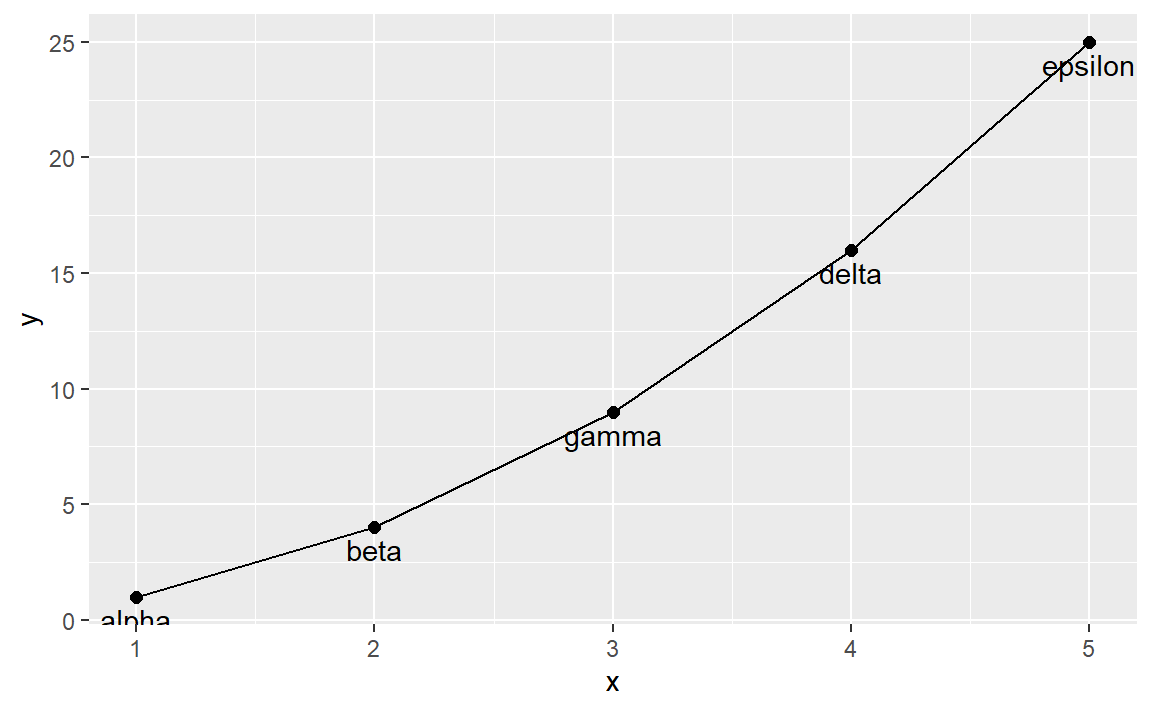
\includegraphics{happy-visualization_files/figure-latex/data_frame-love-1} \end{center}

\hypertarget{viz-secret-with}{%
\section{\texorpdfstring{다른 접근방식 \texttt{with()}}{다른 접근방식 with()}}\label{viz-secret-with}}

데이터프레임을 시각화 입력으로 삼는 전략의 우수성을 기존 다른 접근법과 비교해보자.
슬프게도 모든 함수가 \texttt{data=} 인자를 제공하지는 않는다.
상관계수를 계산하는 \texttt{cor()} 함수를 예로 들어보자. 다음 코드는 동작하지 않는다:

물론 다음과 같이 데이터프레임 명칭을 항상 반복하면 원하는 결과를 얻을 수 있다.

\begin{verbatim}
## [1] 0.436
\end{verbatim}

하지만, \texttt{gapminder}를 두번 타이핑하게 되어 중복 반복 작업이 있어
사람들이 싫어한다. 아마도 이렇게 \texttt{gapminder}를 반복적으로 타이핑한다는 의식속에 숨겨진 공포가
작업공간에 독립된 객체에 변수를 복사하게 만든 동기가 되지 않았나 싶다.

\texttt{with()} 함수가 이런 문제를 피해나가는 해결책이 된다.
데이터프레임을 첫번째 인자로 넣는다.
두번째 인자는 특별히 격리된 환경에서 평가되는 표현식이 된다.
명령어 한줄 혹은 여러줄로 된 토막 코드가 될 수도 있다.
특별한 점은 데이터프레임에 변수를 이름으로 참조할 수 있다는 것이다.

\begin{verbatim}
## [1] 0.436
\end{verbatim}

\texttt{magrittr} 팩키지를 사용하게 되면, 또다른 선택욥션이 \texttt{\%\$\%} 연산자를 사용해서 데이터프레임 내부 변수를 노출시켜 향후 연산작업을 진행해 나가는 방식도 있다. 참고로 \texttt{magrittr} 패키지의 영감을 얻어
\texttt{tiydverse} 생태계를 연결하는 \texttt{\%\textgreater{}\%} 이 생겨났다.

\begin{verbatim}
## [1] 0.436
\end{verbatim}

\hypertarget{viz-secret-case-study}{%
\section{사례}\label{viz-secret-case-study}}

특정한 국가 예를 들어 한국을 뽑아 연도별로 모든 정량적 변수를 도식화한다.

본능적으로 먼저 \texttt{gapminder} 데이터에서 한국을 뽑아 변수별로 루프를 돌려서
개별적으로 그림을 그리고 이를 한데 묶는다.
사실 이러한 방식으로도 작업을 수행할 수 있다.
하지만, 데이터 형태를 바꾸는 방식이 루프를 돌리는 것보다 현재 R 생태계를 고려하면 좀더 ``R스럽다''.

\hypertarget{viz-secret-case-study-data}{%
\subsection{데이터 형태 바꾸기}\label{viz-secret-case-study-data}}

먼저 \texttt{gapminder} 데이터에서 한국만 뽑아낸다.
그리고 나서 \texttt{pop}, \texttt{lifeExp}, \texttt{gdpPercap} 변수를 \texttt{var} 동반변수를 키로
\texttt{value} 변수를 값으로 하여 변수하나로 \texttt{gather()}함수를 통해 모은다.

\begin{verbatim}
## [1] 12  6
\end{verbatim}

\begin{verbatim}
## [1] 36  5
\end{verbatim}

필터링된 \texttt{korea\_dat}는 12 행을 갖는다.
\texttt{korea\_tidy} 데이터프레임에 변수를 세개 모아 쌓아서, 행의 갯수가 3 배 되는 것이 이해된다.
즉, 폭이 넓은 데이터를 길이가 긴 데이터로 바꿔서 36 행을 갖는다.

\hypertarget{viz-secret-case-study-facet}{%
\subsection{\texorpdfstring{\texttt{facet} 기능으로 변수를 반복}{facet 기능으로 변수를 반복}}\label{viz-secret-case-study-facet}}

데이터가 깔끔한 데이터프레임에 반복을 돌릴 수 있는 변수를 나타내는 적절한 요인으로 구성되어서,
\texttt{facet} 기능을 구현하기만 하면 된다.

\begin{center}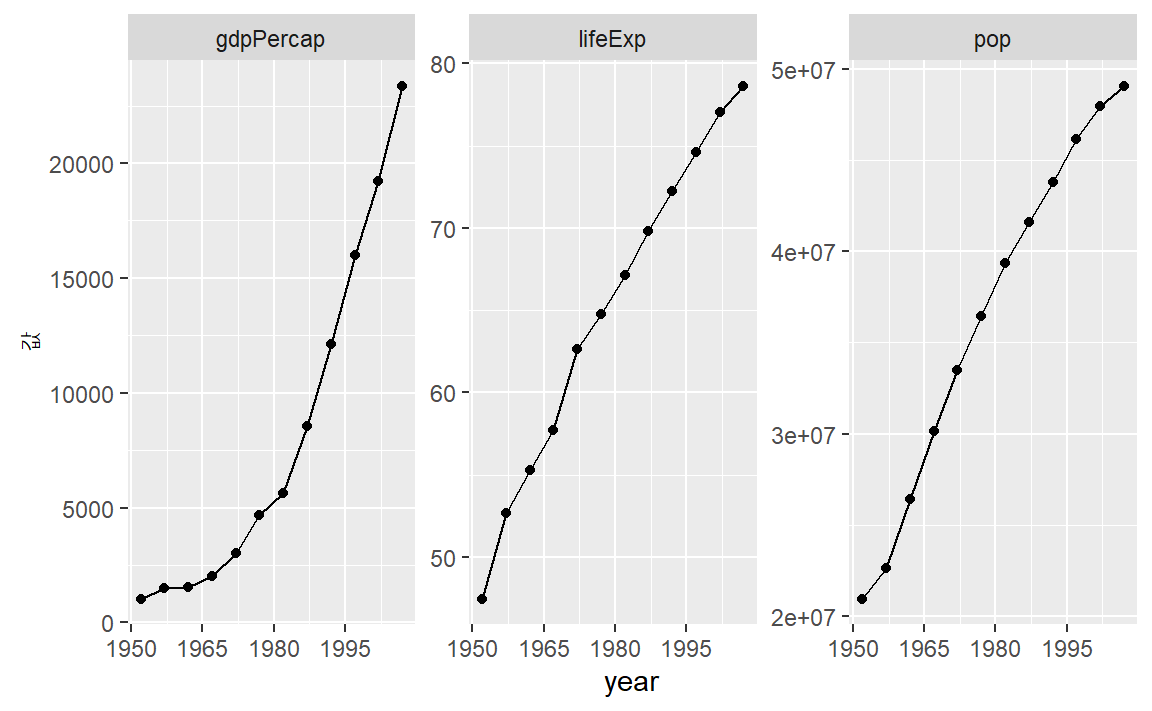
\includegraphics{happy-visualization_files/figure-latex/korea-facet-1} \end{center}

\hypertarget{viz-secret-summary}{%
\subsection{요약}\label{viz-secret-summary}}

한국을 뽑아 시각화한 코드가 다음에 요약되어 있다.

앞에서 언급한 규칙에서 나온 이득을 상기 토막 코드가 보여주고 있다.

\begin{itemize}
\tightlist
\item
  한국만 \texttt{dplyr} 패키지 \texttt{filter()} 함수 데이터 조작을 통해 시각화 \textbf{데이터프레임}으로 독립.
\item
  데이터를 \textbf{폭넓은(wide) → 긴(long)} 형태로 바꾼 전형적인 \textbf{깔끔화} 사례.

  \begin{itemize}
  \tightlist
  \item
    칼럼 세개를 칼럼 한개로 모으는데 이유는 그림에 \texttt{y}-축에 각 변수를 도식화에 용이.
  \end{itemize}
\item
  각 작은 그림(facet)에 속한 관측점을 구별하는데 \textbf{범주}(\texttt{변수})을 사용하고 나서, 패싯 기능 적용.
\end{itemize}

\end{document}
